
\section{Setup}

    \textbf{Hello World!} test \LaTeX. %notice how the command will end at the first non-alphabet charecter such as the . after \LaTeX
    \LaTeX{} is a great program for writing math. I can write in line math such as $a^2+b^2=c^2$ %$ tells LaTexX to compile as math
    . I can also give equations their own space: 
    \begin{equation} % Creates an equation environment and is compiled as math
    \gamma^2+\theta^2=\omega^2
    \frac{12}{12}
    \end{equation}
    If I do not leave any blank lines \LaTeX{} will continue  this text without making it into a new paragraph.  Notice how there was no indentation in the text after equation (1).  
    Also notice how even though I hit enter after that sentence and here $\downarrow$
    \LaTeX{} formats the sentence without any break.  Also   look  how      it   doesn't     matter          how    many  spaces     I put     between       my    words.

    For a new paragraph I can leave a blank space in my code. 
    
        \begin{figure}[!htb]
            \centering
            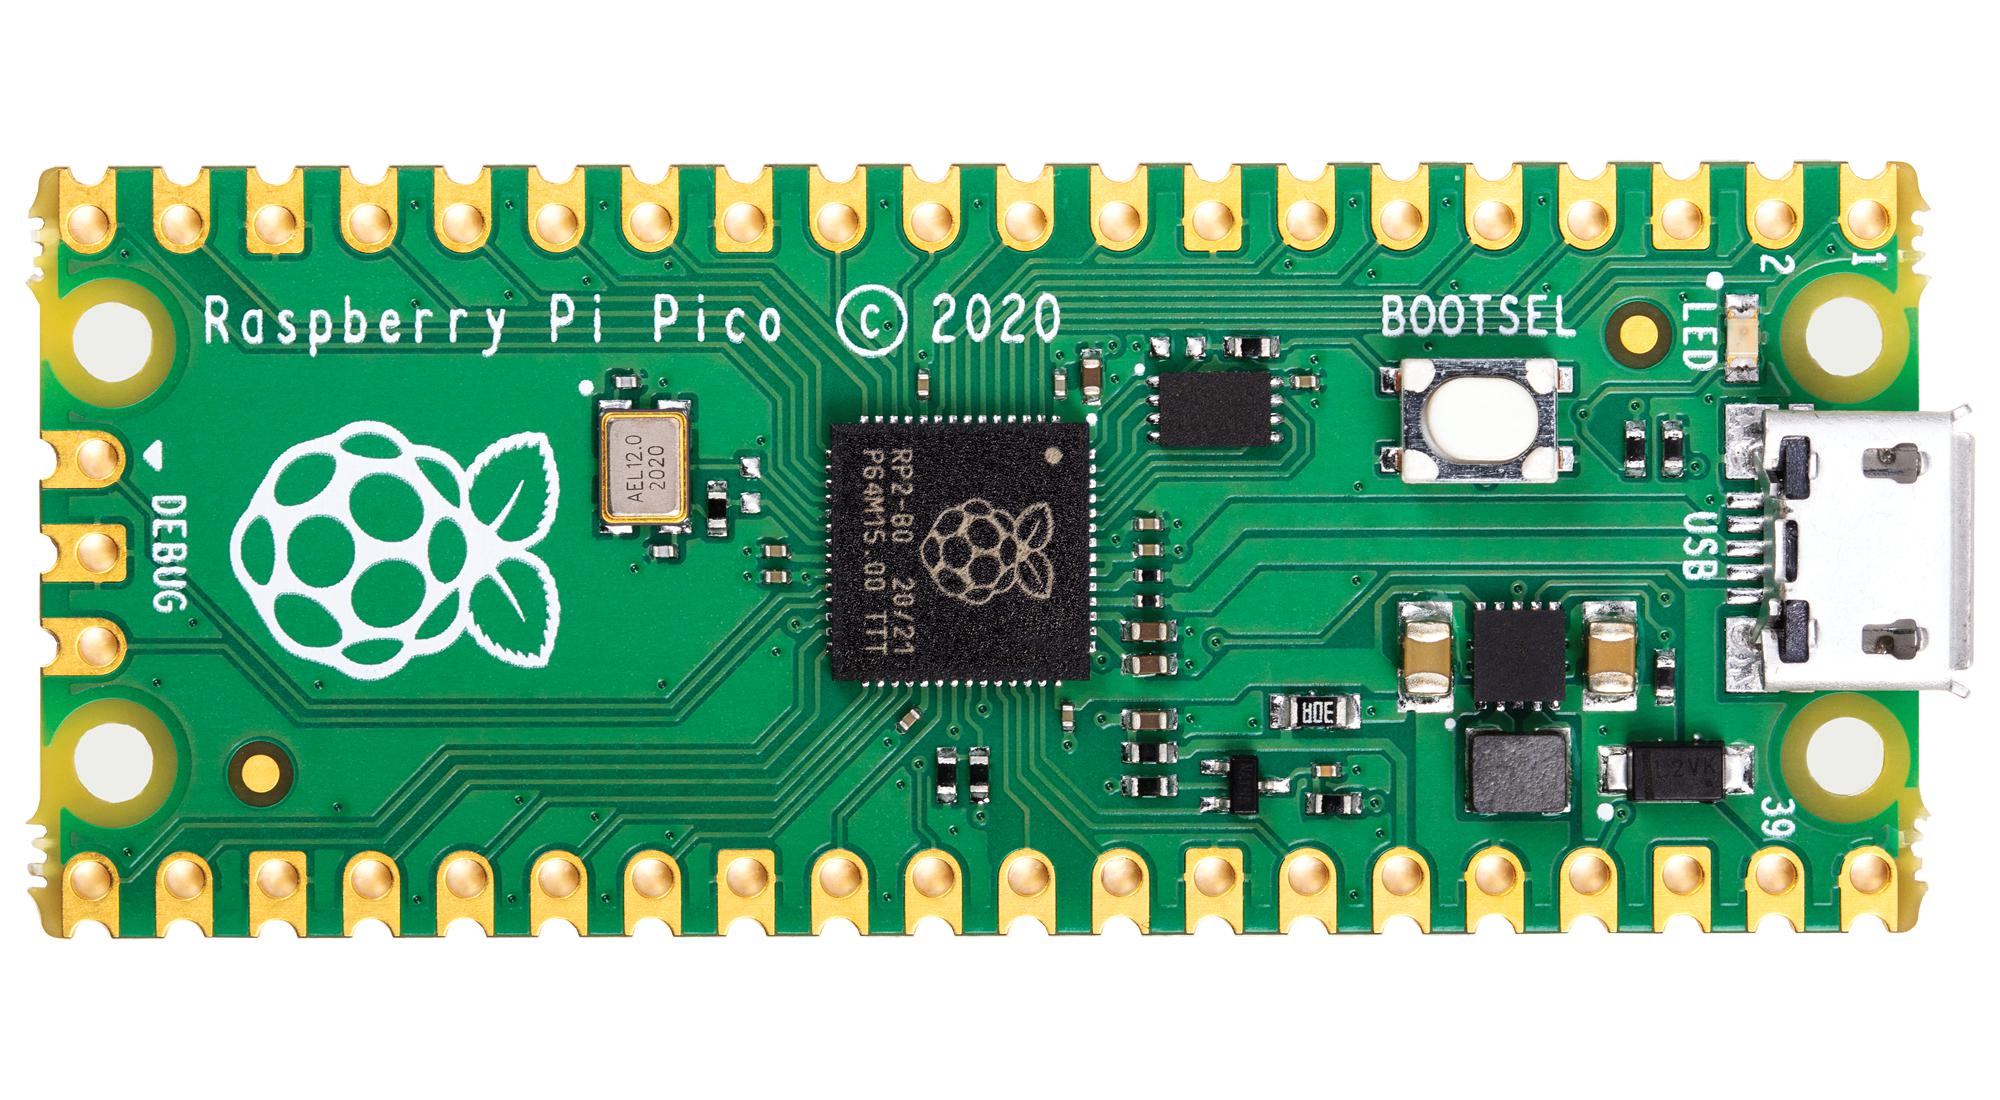
\includegraphics[width=0.5\textwidth]{pi}
            \caption{Płytka rasebrry Pi.}
        \end{figure}


\subsection{Problemy}
Poprzez nieprawidłowe ułożenie tekstu trenowałem bardzo dużo\\
\href{url}{http://www.texample.net/tikz/resources/}



